
\section{Graphic novel design example}

\begin{figure}[H]
\fbox{% start a box
  \parbox{1\textwidth}{% create a paragraph box of 0.8 times the text width
\begin{alltt}
\small
I would like to write a one page graphic novel for little girls, do you have any idea of what I could do? \\

\lightgreen{ Possible one page graphic novels for little girls:

- A girl who loves to draw discovers a magic crayon that brings her creations to life, and uses it to make friends with a unicorn, a dragon, and a fairy.

- A girl who dreams of becoming a detective solves a mystery at her school, finding clues, suspects, and a hidden treasure in the library, the cafeteria, and the playground.

- A girl who is afraid of the dark learns to overcome her fear with the help of a friendly star, who guides her through a nighttime adventure full of wonders and surprises.

- A girl who loves to bake enters a contest to create the most delicious and original cupcake, and faces challenges, rivals, and judges along the way, but also finds support and inspiration from her family and friends.

- A girl who wants to play soccer with the boys proves her skills and courage by joining a secret league of girls who play at night, wearing masks and capes, and using special moves and gadgets. } \\

I love the first idea, let's make it even simpler, just a girl who loves to draw and discovers a magic crayon that she uses to bring a unicorn to life. Can you help me realizing that one page graphic novel? \\

\lightgreen{ Possible steps to realize that one page graphic novel:

- Sketch out a rough layout of the page, dividing it into panels of different sizes and shapes according to the flow of the story. For example, you could use a large panel for the opening scene, where the girl is drawing in her room, then smaller panels for the moments when she finds the magic crayon, draws the unicorn, and sees it come to life, and then a final large panel for the ending scene, where she hugs the unicorn and smiles.

- Write the dialogue and captions for each panel, using simple and expressive language that matches the tone and mood of the story. For example, you could use a caption to introduce the girl and her hobby, then have her say things like "Wow, what a cool crayon!", "I wish I had a unicorn friend", and "You're real!" to show her curiosity, desire, and joy. You could also use sound effects to add some drama and humor, such as "Scribble, scribble", "Poof!", and "Neigh!"

- Draw the characters and backgrounds for each panel, using a clear and colorful style that appeals to little girls. For example, you could make the girl cute and expressive, with big eyes, long hair, and a dress, and the unicorn majestic and friendly, with a horn, a mane, and a tail. You could also add some details and accessories to make them more unique and interesting, such as a flower in the girl's hair, a star on the unicorn's forehead, or a poster of a fairy tale on the wall. }
\end{alltt}}}
\end{figure}

\begin{figure}[H]
\fbox{% start a box
  \parbox{1\textwidth}{% create a paragraph box of 0.8 times the text width
\begin{alltt}
\small
\lightgreen{ - Ink and color the panels, using a pen, a brush, or a digital tool to outline and fill in the shapes and textures. For example, you could use black ink for the outlines, and bright colors for the characters and backgrounds, such as pink, purple, and blue. You could also use some shading, highlights, and patterns to create some depth and contrast, such as a gradient for the sky, a sparkle for the magic crayon, or a stripe for the unicorn's coat.

- Add the dialogue and captions, using a font, a lettering, or a handwriting that fits the style and voice of the story. For example, you could use a round and bubbly font for the girl's speech, and a script and elegant font for the captions, and place them in balloons and boxes that match the shape and size of the panels. You could also use some effects and variations to emphasize some words or emotions, such as a bold or italic font, a bigger or smaller size, or a different color or shape. } \\

That sounds really amazing. Can you write SVG code that produces this one page graphic novel? \\

\lightgreen{ SVG code is a markup language that can be used to create vector graphics, such as shapes, paths, text, and filters. However, writing SVG code by hand can be quite tedious and complex, especially for a one page graphic novel with multiple panels, characters, backgrounds, and effects. Therefore, it might be easier and faster to use a graphical editor or a software tool that can generate SVG code from a visual input, such as Inkscape, Adobe Illustrator, or SVG-edit. Alternatively, one could use another format or language that can be converted to SVG, such as HTML, CSS, or JavaScript, and use a library or a framework that can handle the conversion, such as D3.js, Snap.svg, or SVG.js.

Nonetheless, here is a possible example of SVG code that could produce a simplified version of the one page graphic novel, based on the steps above. Note that this code is not optimized or complete, and may not work properly in all browsers or contexts. It is also not very readable or maintainable, and would benefit from some refactoring and commenting. It is only meant to illustrate the general structure and syntax of SVG code, and how it could be used to create a basic comic page. [Output of SVG code below.] }
\end{alltt}}}
\end{figure}

\begin{figure}[h]
	\centering
	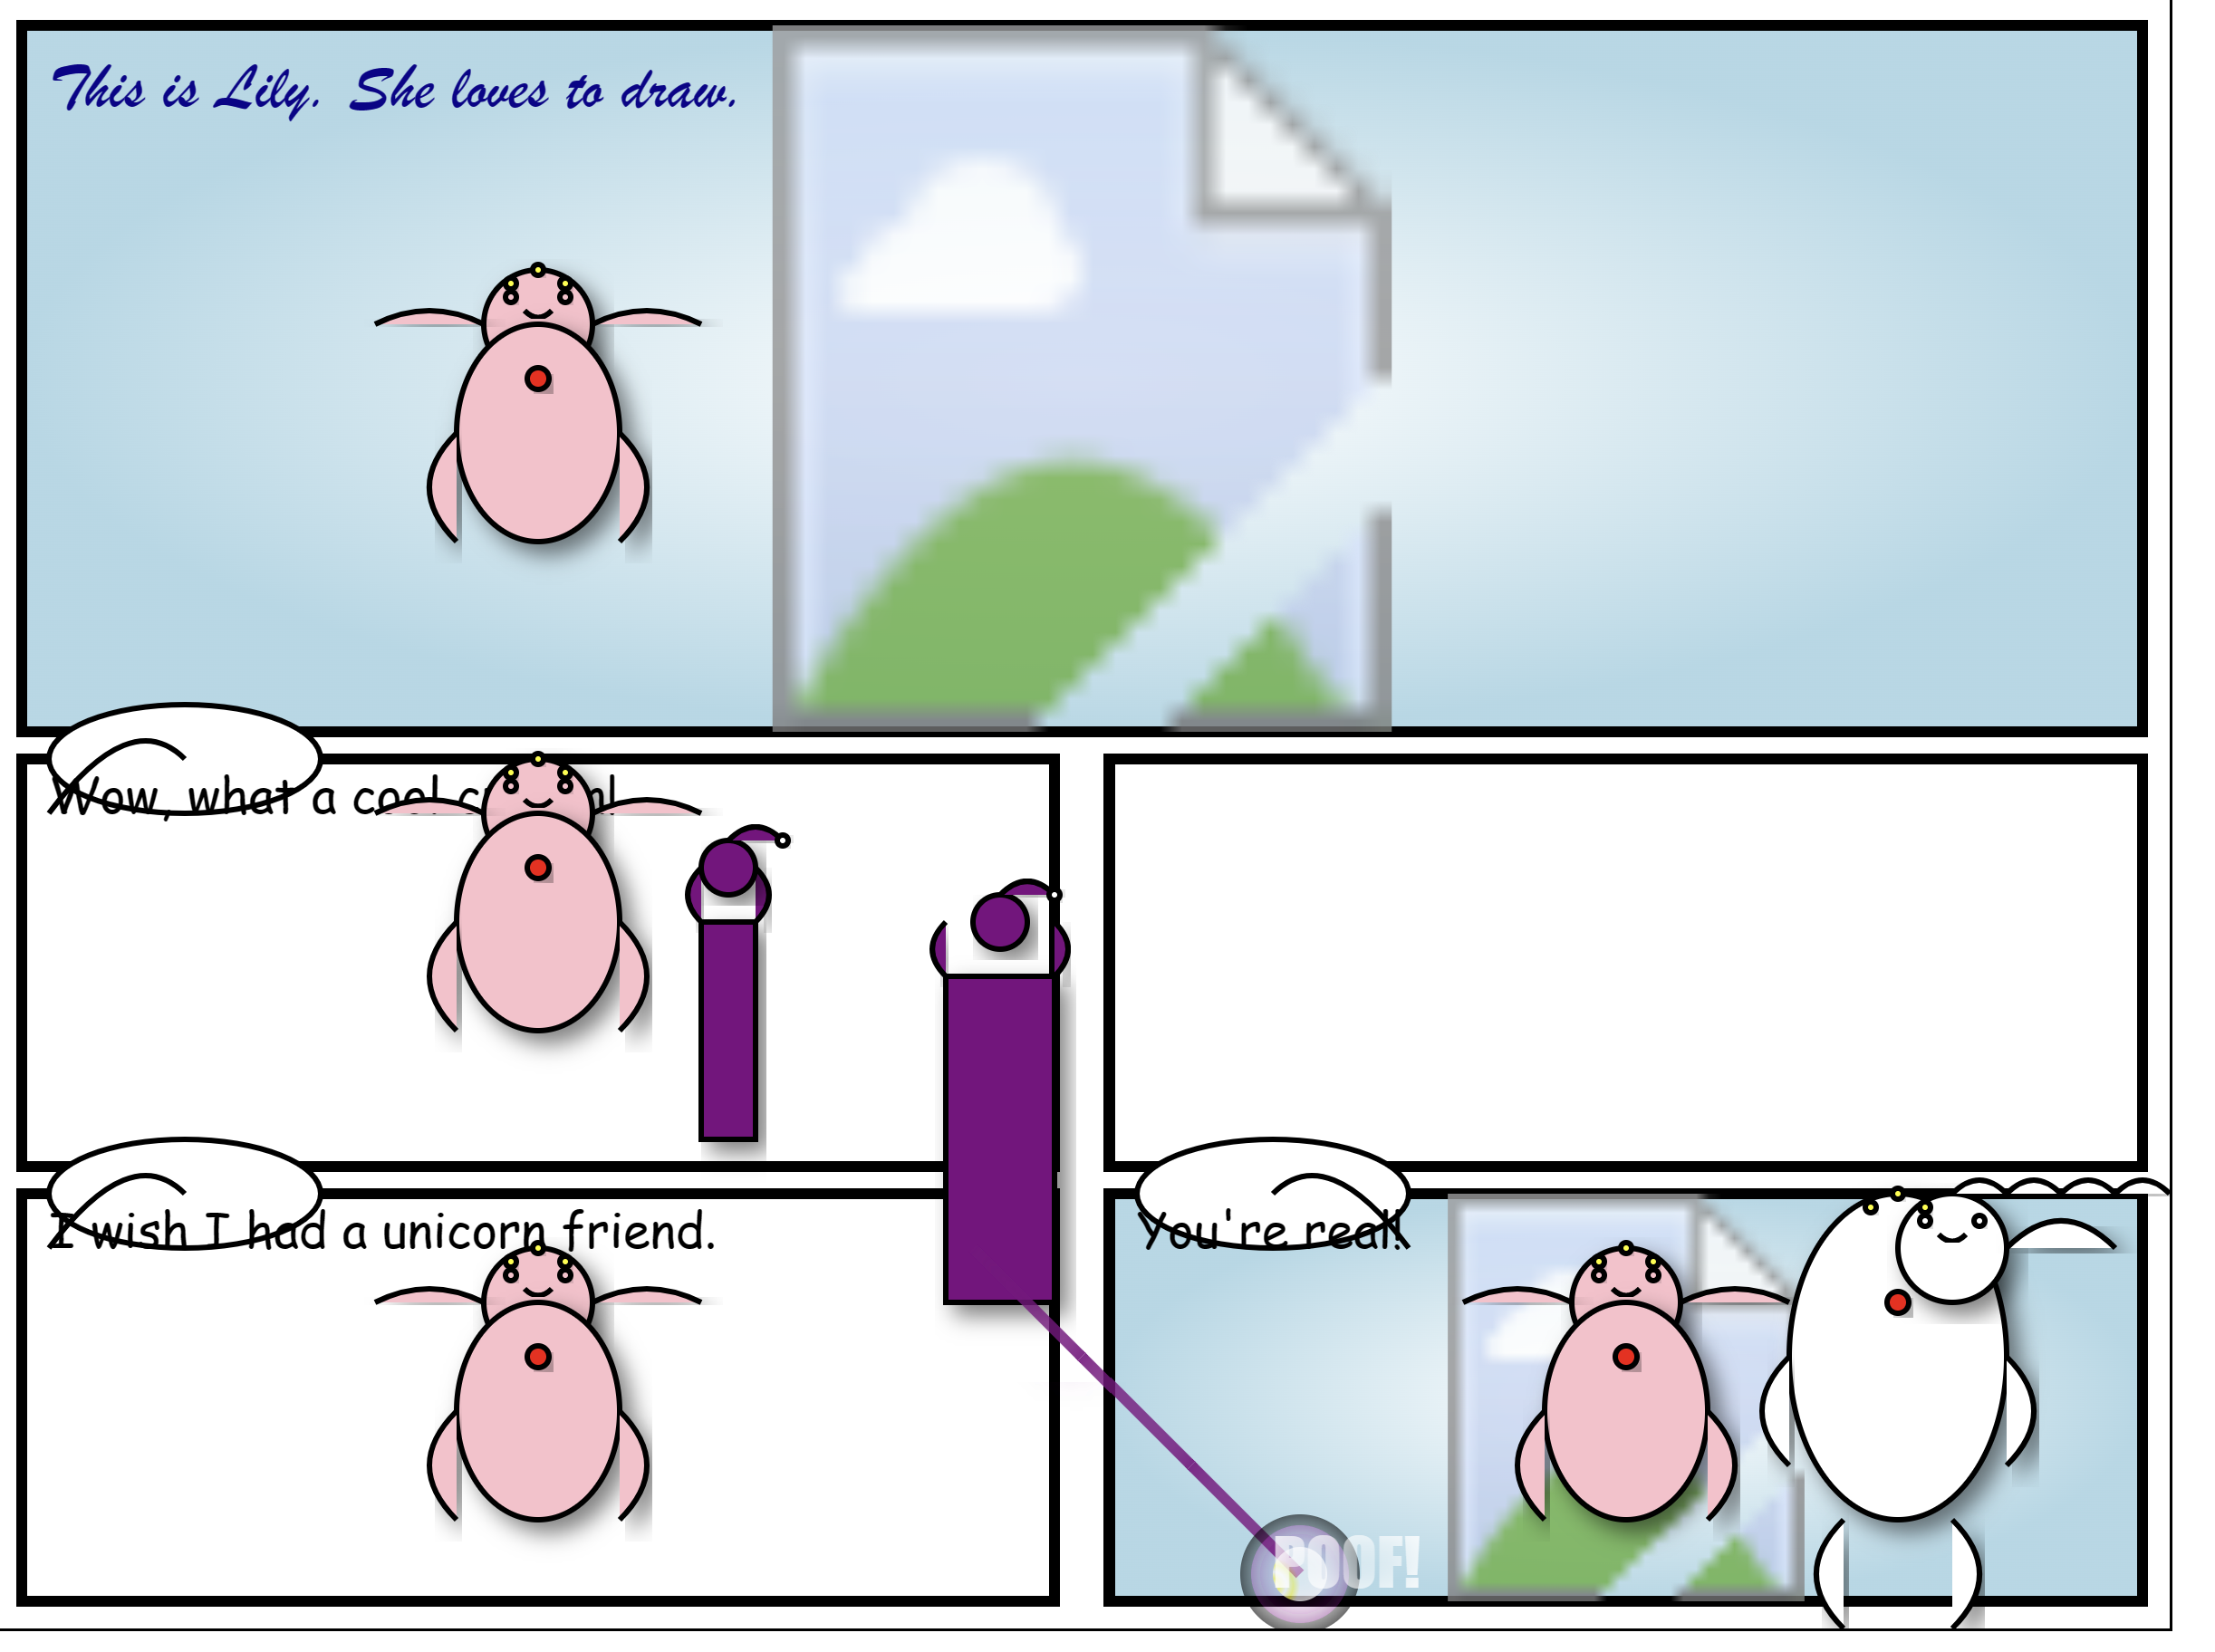
\includegraphics[width=0.55\textwidth]{figures/novel.png}
	\label{fig:novel}
\end{figure}


